\documentclass[10pt]{article}

% ---------- layout & typography ----------
\usepackage[letterpaper,margin=1in,headheight=14pt]{geometry}
\usepackage{lmodern}
\usepackage[T1]{fontenc}
\usepackage[utf8]{inputenc}
\usepackage{microtype}
\usepackage{parskip}
\emergencystretch=1.5em
\usepackage{enumitem}
\setlist{nosep,leftmargin=1.4em}
\usepackage{titlesec}
\titleformat{\section}{\Large\bfseries\sffamily}{\thesection}{0.8em}{}
\titleformat{\subsection}{\large\bfseries\sffamily}{\thesubsection}{0.8em}{}
\titleformat{\subsubsection}{\normalsize\bfseries\sffamily}{\thesubsubsection}{0.8em}{}
\usepackage{fancyhdr}
\pagestyle{fancy}
\fancyhf{}
\fancyhead[L]{\small\sffamily Veloce PQC SDK: V1 Engineering Plan}
\fancyhead[R]{\small\sffamily Lightrider Inc (Confidential)}
\fancyfoot[C]{\small\thepage}

% ---------- tables, color, graphics ----------
\usepackage{booktabs}
\usepackage{tabularx}
\usepackage{ltablex}   % makes tabularx breakable across pages
\keepXColumns
\usepackage{array}
\usepackage{xcolor}
\definecolor{lrblue}{RGB}{22,80,145}
\definecolor{lrgray}{RGB}{100,108,116}
\definecolor{warnred}{RGB}{176,42,32}
\definecolor{okgreen}{RGB}{22,120,70}
\definecolor{fipsgold}{RGB}{150,110,20}
\usepackage{tikz}
\usetikzlibrary{positioning,fit,arrows.meta,calc}
\usepackage{hyperref}
\hypersetup{colorlinks=true,linkcolor=lrblue,urlcolor=lrblue,citecolor=lrblue,
  pdftitle={Veloce PQC SDK V1 Engineering Plan},pdfauthor={Lightrider Inc}}

% ---------- mini vector icons (pure TikZ, scale with text) ----------
\newcommand{\icPy}{\tikz[baseline=-2.4pt]{%
  \draw[lrblue, line width=0.8pt] (-1.0pt,2.2pt) -- (-2.8pt,0) -- (-1.0pt,-2.2pt);
  \draw[lrblue, line width=0.8pt] (1.0pt,2.2pt) -- (2.8pt,0) -- (1.0pt,-2.2pt);
  \draw[lrblue, line width=0.6pt] (0.7pt,2.8pt) -- (-0.7pt,-2.8pt);}}
\newcommand{\icTerm}{\tikz[baseline=-2.4pt]{%
  \draw[lrblue, line width=0.7pt, rounded corners=0.8pt] (-3.4pt,-2.6pt) rectangle (3.4pt,2.6pt);
  \draw[lrblue, line width=0.8pt] (-2.2pt,1.1pt) -- (-0.9pt,0) -- (-2.2pt,-1.1pt);
  \draw[lrblue, line width=0.8pt] (0pt,-1.3pt) -- (2.2pt,-1.3pt);}}
\newcommand{\icSearch}{\tikz[baseline=-2.4pt]{%
  \draw[lrblue, line width=0.9pt] (-0.6pt,0.6pt) circle (2.1pt);
  \draw[lrblue, line width=1.1pt] (0.9pt,-0.9pt) -- (2.8pt,-2.8pt);}}
\newcommand{\icGear}{\tikz[baseline=-2.4pt]{%
  \draw[lrblue, line width=0.7pt] (0,0) circle (1.2pt);
  \draw[lrblue, line width=0.7pt] (0,0) circle (2.3pt);
  \foreach \a in {0,45,...,315} \draw[lrblue, line width=0.9pt] (\a:2.3pt) -- (\a:3.3pt);}}
\newcommand{\icShield}{\tikz[baseline=-2.6pt]{%
  \draw[fipsgold, line width=0.8pt] (-2.6pt,2.4pt) -- (0,3.2pt) -- (2.6pt,2.4pt) -- (2.6pt,-0.4pt)
    .. controls (2.6pt,-2.0pt) and (1.2pt,-3.0pt) .. (0,-3.6pt)
    .. controls (-1.2pt,-3.0pt) and (-2.6pt,-2.0pt) .. (-2.6pt,-0.4pt) -- cycle;
  \draw[fipsgold, line width=0.7pt] (-1.1pt,0.2pt) -- (-0.2pt,-0.9pt) -- (1.3pt,1.1pt);}}
\newcommand{\icWave}{\tikz[baseline=-1.4pt]{%
  \draw[fipsgold, line width=0.8pt]
    (0,0) -- (0.9pt,0) -- (1.5pt,2.0pt) -- (2.6pt,-2.0pt) -- (3.4pt,1.2pt) -- (4.2pt,-0.8pt)
    -- (4.8pt,0) -- (5.8pt,0);}}
\newcommand{\icAtom}{\tikz[baseline=-1.8pt]{%
  \fill[lrblue] (0,0) circle (0.7pt);
  \draw[lrblue, line width=0.5pt] (0,0) ellipse (3.2pt and 1.3pt);
  \draw[lrblue, line width=0.5pt, rotate=60] (0,0) ellipse (3.2pt and 1.3pt);
  \draw[lrblue, line width=0.5pt, rotate=120] (0,0) ellipse (3.2pt and 1.3pt);}}
\newcommand{\icCloud}{\tikz[baseline=-2.0pt]{%
  \draw[lrgray, line width=0.8pt, fill=lrgray!10]
    (-2.6pt,-1.2pt) .. controls (-4.0pt,-1.2pt) and (-4.0pt,1.0pt) .. (-2.4pt,1.0pt)
    .. controls (-2.2pt,2.6pt) and (0.6pt,2.8pt) .. (1.0pt,1.4pt)
    .. controls (2.8pt,1.8pt) and (3.4pt,-0.2pt) .. (2.2pt,-1.2pt) -- cycle;}}
\newcommand{\icLock}{\tikz[baseline=-2.2pt]{%
  \draw[lrblue, line width=0.8pt, rounded corners=0.5pt] (-2.2pt,-3.0pt) rectangle (2.2pt,0.2pt);
  \draw[lrblue, line width=0.8pt] (-1.3pt,0.2pt) -- (-1.3pt,1.4pt) arc (180:0:1.3pt) -- (1.3pt,0.2pt);
  \fill[lrblue] (0,-1.4pt) circle (0.6pt);}}

% ---------- inline tags ----------
\newcommand{\dep}[1]{\textcolor{warnred}{\sffamily\bfseries\small [VENDOR: #1]}}
\newcommand{\open}[1]{\textcolor{fipsgold}{\sffamily\bfseries\small [OPEN: #1]}}
\newcommand{\decided}[1]{\textcolor{okgreen}{\sffamily\bfseries\small [DECIDED: #1]}}
\newcommand{\code}[1]{\texttt{\small #1}}

\newcolumntype{L}{>{\raggedright\arraybackslash}X}

\begin{document}

% =====================================================================
\begin{titlepage}
\centering
{\Huge\sffamily\bfseries Veloce}\\[0.4em]
{\LARGE\sffamily Post-Quantum Cryptography SDK}\\[2.5em]
{\huge\sffamily\bfseries V1 Engineering Plan}\\[3em]
\begin{tabular}{ll}
\toprule
Organization & Lightrider Inc \\
Product & Veloce: cryptographic search SDK + FIPS entropy generator \\
Version & 0.1 (draft for review) \\
Date & August 4, 2026 \\
Prepared for & Martin Guo, Quantum Applied Scientist \\
Status & Awaiting stakeholder feedback \\
\bottomrule
\end{tabular}
\vfill
\begin{minipage}{0.85\textwidth}
\small\sffamily
\textbf{Abstract.} Veloce V1 delivers two products in one SDK:
\textbf{qSearch}, a high-performance cryptographic discovery tool (source, dependencies,
certificates, network) that produces a Cryptography Bill of Materials (CBOM) on
Windows~11 and Linux x86-64; and the \textbf{Veloce crypto core}, a locally deployed
entropy generator and PQC service built on the wolfCrypt FIPS~140-3 module
(certificate \#4718) seeded exclusively by wolfSSL's ESV-certified wolfEntropy source,
exposing ML-KEM, ML-DSA, and hybrid TLS~1.3 through a Python SDK. Cloud connectivity to
the Lightrider EMS is optional, off by default, and includes a user-controllable cloud-entropy
mix-in that never weakens the local FIPS entropy claim.
\end{minipage}
\vspace{2em}
\end{titlepage}

\tableofcontents
\newpage

% =====================================================================
\section{Executive Summary}\label{sec:exec}

Veloce is Lightrider's V1 PQC SDK. It comprises a cryptographic discovery component
(qSearch) and a FIPS 140-3 crypto core with a validated entropy pipeline. Both operate
fully offline; an optional EMS connection provides fleet telemetry and user-controlled
cloud entropy.

\textbf{Document organization.} This document is the implementation specification for
Veloce V1 and is sufficient for reimplementation on its own. Sections
\ref{sec:arch}--\ref{sec:ems} define the components, Section~\ref{sec:api} the public
API and deliverables, Section~\ref{sec:security} the security controls,
Section~\ref{sec:gates} the acceptance tests, Section~\ref{sec:schedule} the build order
with a component-to-repository map, and the appendices the exact build commands.

\subsection*{The two pillars}
\begin{description}[style=nextline]
  \item[Pillar A: qSearch (cryptographic search).] A Rust-based discovery engine with
  replaceable open-source collectors (CryptoScan, Zeek/Suricata, TShark+Npcap). It finds
  RSA, DH, ECDH, ECDSA and other quantum-vulnerable usage in source code, dependencies,
  certificates, and network traffic, and emits JSON, CSV, CycloneDX CBOM, and
  OMB M-23-02 inventory fields. Lightrider owns the normalization, correlation,
  classification, CBOM generation, risk scoring, and reporting layers.
  \item[Pillar B: Entropy generator and FIPS crypto core.] A native C++17 agent embedding
  the wolfCrypt FIPS 140-3 validated module (CMVP cert \#4718) whose SP~800-90A Hash\_DRBG
  is seeded only by wolfSSL's ESV-certified wolfEntropy source (SP~800-90B health tests,
  fail-closed). The agent provides ML-KEM-768 key establishment, ML-DSA signatures, and
  hybrid TLS 1.3, consumed from a pure-Python SDK over an authenticated local IPC channel.
\end{description}

\subsection*{Technical stack}

The product is designated \textbf{Veloce}; its components are qSearch, the Veloce Agent,
the Veloce Python SDK, the Veloce CLI, and EMS (\code{light-rider-platform}).

\begin{small}
\begin{tabularx}{\textwidth}{@{}l>{\raggedright\arraybackslash}p{0.33\textwidth}L@{}}
\toprule
\textbf{Layer} & \textbf{Stack element} & \textbf{Technical basis} \\
\midrule
Crypto module & wolfCrypt FIPS 140-3 module v5.2.1, CMVP cert \#4718, dynamically
  loaded & The guidance mandates a shared library/DLL (no static linking) and the
  purchased bundle carries this exact validated module; autotools
  (\code{-{}-enable-fips=v5}) is its only FIPS-capable build path. \\
Entropy source & wolfEntropy (ESV), \code{-{}-enable-wolfEntropy=nofallback}, wired via
  \code{wc\_SetSeed\_Cb()} & The FIPS module itself makes no entropy claim; SP~800-90B
  compliance therefore requires an external ESV-validated source, which the bundle
  provides with built-in RCT/APT health tests. V1 entropy is software-only; hardware
  QRNG (IDQ Quantis) and the Quantropi quantum-entropy service are post-V1
  integrations. \\
PQC provider & ML-KEM / ML-DSA compiled \emph{beside} the FIPS boundary & The v5 FIPS
  build strips SHAKE/XOF from in-boundary SHA-3, so FIPS 203/204 code cannot link inside
  it; reported as \code{pqc\_inside\_fips\_boundary:\ false} until wolfSSL's FIPS v7
  ``PQ-FS'' module ships (Section~\ref{sec:pqc-boundary}). \\
Agent & C++17 native service & The Windows instruction set specifies C++17; wolfCrypt is
  a C library, making C++ the lowest-friction FFI; all keys and FIPS state must reside in
  one local process. \\
qSearch & Rust & Parsing-heavy, parallel scanning across untrusted inputs favors a
  memory-safe compiled language; it links no wolfCrypt code, so the FFI constraint does
  not apply. \\
SDK client & Pure Python over local IPC & The guidance mandates a pure-Python IPC client
  that never loads the crypto library; private keys are represented only as opaque
  handles. \\
Cloud entropy & EMS-delivered packets as DRBG \emph{additional input}, default off &
  SP~800-90A permits additional input with zero credited entropy, so cloud entropy can
  strengthen output without altering the FIPS/ESV claims; the source documents prohibit
  entropy leaving the device, and this design sends none. \\
Platforms & Windows 11 x86-64; Linux x86-64 & Fixed by the V1 scope statement
  (``Start with Windows and Linux only''); macOS deferred. \\
Licensing & Lightrider commercial EULA wrapping the wolfSSL commercial license & The
  agreement (v.01-24) permits object-code redistribution of the Combined Program with
  notices retained (Section~\ref{sec:license}). \\
\bottomrule
\end{tabularx}
\end{small}

\subsection*{Terminology}

\begin{small}
\begin{tabularx}{\textwidth}{@{}lL@{}}
\toprule
\textbf{Term} & \textbf{Meaning in this document} \\
\midrule
PQC & Post-quantum cryptography: algorithms that resist attack by quantum computers. \\
Quantum-vulnerable & Cryptography a large quantum computer could break: RSA, DH, ECDH,
  ECDSA. \\
ML-KEM / ML-DSA & The NIST-standardized post-quantum key-establishment (FIPS 203) and
  signature (FIPS 204) algorithms. \\
Hybrid TLS & A TLS 1.3 handshake combining a classical and a post-quantum key exchange;
  secure if either component holds. \\
FIPS 140-3 & The U.S.\ government standard for validating cryptographic modules;
  validation is issued as a numbered CMVP certificate. \\
Module boundary & The exact code covered by a FIPS certificate; anything outside it
  carries no validation claim. \\
OE & Operational environment: the specific operating system and hardware a validation
  was tested on. \\
Entropy & Unpredictable data used to seed random-number generation; the root of all key
  security. \\
ESV & NIST Entropy Source Validation: certifies an entropy source under SP~800-90B. \\
DRBG & Deterministic random bit generator: expands a small entropy seed into unlimited
  random output (SP~800-90A). \\
RCT / APT & The two continuous entropy health tests (repetition count, adaptive
  proportion) required by SP~800-90B. \\
KAT / CAST & Known-answer test / conditional algorithm self-test: fixed-input checks a
  FIPS module runs on its own algorithms. \\
CBOM / SBOM & Cryptography / software bill of materials: an inventory of where and how
  cryptography (or software) is used. \\
Collector & A replaceable tool qSearch uses to gather raw evidence (source scan,
  certificate scan, network capture). \\
Correlate & Merge findings from different collectors that refer to the same asset. \\
Remediation & Changing or replacing vulnerable cryptography; V1 discovers and reports
  only. \\
IPC & Inter-process communication: the authenticated local channel between the Python
  SDK/CLI and the agent. \\
EMS & Lightrider's cloud platform (\code{light-rider-platform}) for fleet telemetry and
  cloud entropy. \\
M-23-02 & The U.S.\ federal memorandum requiring agencies to inventory quantum-vulnerable
  cryptography. \\
\bottomrule
\end{tabularx}
\end{small}

% =====================================================================
\section{Scope and Requirements}\label{sec:scope}

Scope is fixed by the PQC SDK guidance documents and the qSearch architecture notes.
The single V1 scope change approved by Lightrider is the cloud-entropy mix-in
(Section~\ref{sec:ems}).

\subsection{In scope (V1)}
\begin{small}
\begin{tabularx}{\textwidth}{@{}lL@{}}
\toprule
\textbf{Area} & \textbf{V1 capability} \\
\midrule
qSearch discovery & Source-code and dependency scanning; certificate and protocol
  discovery; passive network/PCAP analysis; identification of RSA, DH, ECDH, ECDSA and
  other quantum-vulnerable cryptography \\
CBOM & Automatic CBOM export in JSON, CSV, and CycloneDX; M-23-02 inventory fields;
  executive summary; mapping to the Light Rider CBOM workbook \\
Entropy & wolfEntropy ESV-certified software entropy source, SP~800-90B health tests,
  fail-closed seeding/reseeding of the wolfCrypt DRBG \\
PQC services & ML-KEM key generation / encapsulation / decapsulation; ML-DSA signing /
  verification; opaque key handles only \\
TLS & Hybrid TLS 1.3 (classical + ML-KEM group) sample client and server, policy-profile
  driven (\code{LIGHTRIDER\_PQC\_TRANSITION}) \\
FIPS & Startup + conditional self-tests, approved-mode status, per-item validation-status
  reporting (module cert, ESV cert, PQC status) \\
EMS (optional) & Telemetry/CBOM synchronization; user-controllable cloud-entropy mix-in;
  disabled by default with a zero-network-traffic guarantee \\
Platforms & Windows 11 x86-64 (MSI + Windows service) and Linux x86-64
  (deb/rpm + systemd unit) \\
\bottomrule
\end{tabularx}
\end{small}

\subsection{Out of scope (V1)}
Quantum Light hardware and QPU-derived entropy as \emph{seed} sources; D-QKD; mobile;
tactical hardware; customer-specific FIPS operational environments; multi-source entropy
pooling; proprietary algorithms; automatic remediation/migration orchestration in qSearch;
macOS. \emph{Do not expand V1 scope without approval.}

\subsection{Standards and policy baseline}
\begin{small}
\begin{tabularx}{\textwidth}{@{}llL@{}}
\toprule
\textbf{Standard} & \textbf{Role} & \textbf{Veloce usage} \\
\midrule
FIPS 140-3 & Module validation & wolfCrypt module v5.2.1, CMVP cert \#4718 \\
SP 800-90A & DRBG & Hash\_DRBG (SHA-256), 256-bit strength \\
SP 800-90B / ESV & Entropy source & wolfEntropy: RCT + APT health tests, ESV certificate \\
FIPS 203 / 204 & PQC algorithms & ML-KEM-768 (default), ML-DSA \\
TLS 1.3 (RFC 8446) & Protocol & Hybrid groups, e.g.\ \code{X25519MLKEM768} \\
CycloneDX CBOM & Inventory format & qSearch + SDK CBOM export \\
OMB M-23-02 & Federal policy & Inventory fields; scanning-first CBOM process \\
CISA ACDI strategy & Discovery baseline & Coverage model for qSearch collectors \\
\bottomrule
\end{tabularx}
\end{small}

\open{Federal ``CBOM minimum elements'' are pending; the CBOM schema module must be
versioned so it can adopt them without breaking consumers.}

% =====================================================================
\section{System Architecture}\label{sec:arch}

One native agent owns all keys, entropy, and FIPS state. Python and the CLI are thin,
crypto-free IPC clients. qSearch is a separate Rust binary outside the FIPS boundary that
shares only the CBOM data model with the SDK. EMS is reachable only from the agent, only
when enabled.

\begin{center}
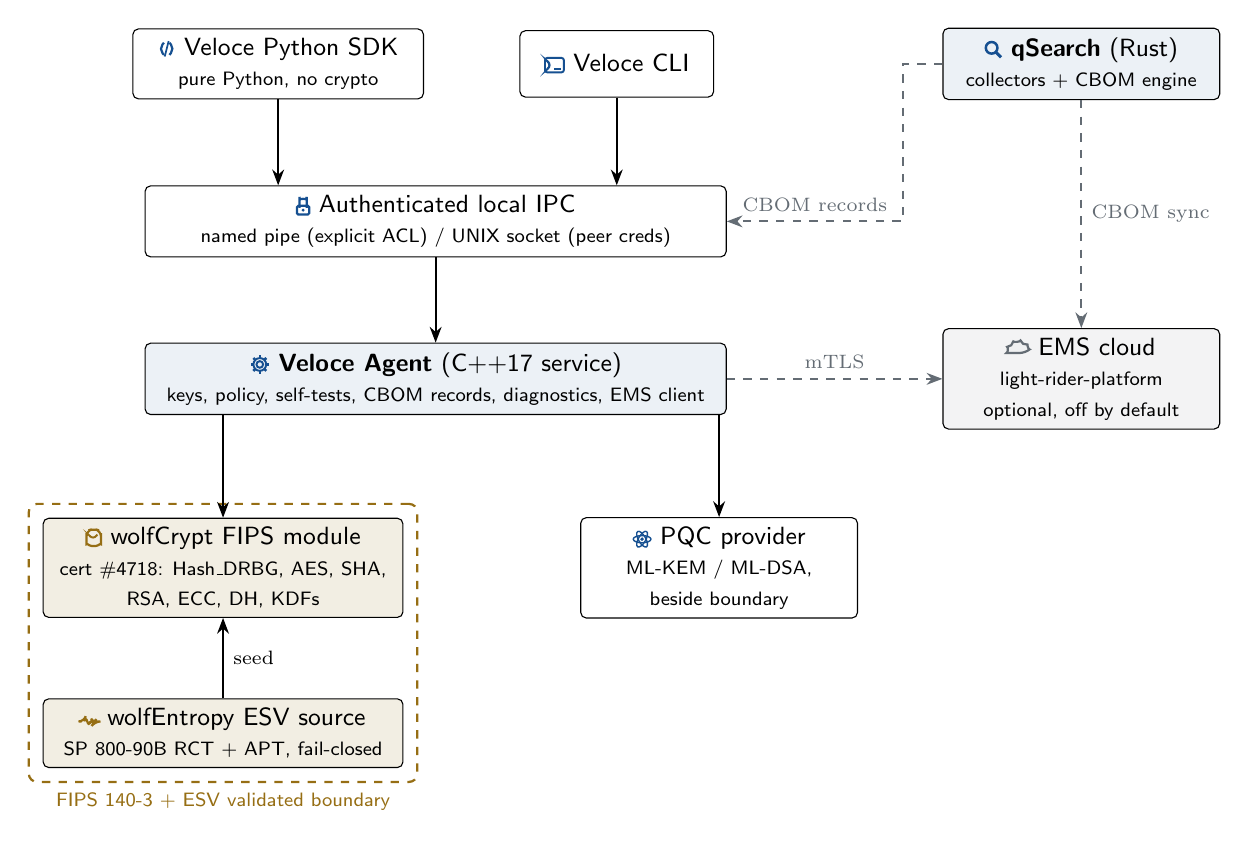
\begin{tikzpicture}[
  font=\small\sffamily,
  box/.style={draw, rounded corners=2pt, minimum height=2.4em, align=center, fill=white},
  arrow/.style={-{Stealth[length=2mm]}, thick},
  dline/.style={-{Stealth[length=2mm]}, thick, dashed, lrgray}]

  % --- client tier (row 0) ---
  \node[box, minimum width=10.5em] (py)  at (0.6,0)   {\icPy\ Veloce Python SDK\\\scriptsize pure Python, no crypto};
  \node[box, minimum width=7em]    (cli) at (4.9,0)   {\icTerm\ Veloce CLI};
  \node[box, fill=lrblue!8, minimum width=10em] (qs) at (10.8,0)
    {\icSearch\ \textbf{qSearch} (Rust)\\\scriptsize collectors + CBOM engine};

  % --- IPC (row 1) ---
  \node[box, minimum width=21em] (ipc) at (2.6,-2.0)
    {\icLock\ Authenticated local IPC\\\scriptsize named pipe (explicit ACL) / UNIX socket (peer creds)};

  % --- agent + EMS (row 2) ---
  \node[box, fill=lrblue!8, minimum width=21em] (agent) at (2.6,-4.0)
    {\icGear\ \textbf{Veloce Agent} (C++17 service)\\\scriptsize keys, policy, self-tests, CBOM records, diagnostics, EMS client};
  \node[box, fill=lrgray!8, minimum width=10em] (ems) at (10.8,-4.0)
    {\icCloud\ EMS cloud\\\scriptsize light-rider-platform\\\scriptsize optional, off by default};

  % --- crypto tier (rows 3-4) ---
  \node[box, fill=fipsgold!12, minimum width=13em] (wc) at (-0.1,-6.4)
    {\icShield\ wolfCrypt FIPS module\\\scriptsize cert \#4718: Hash\_DRBG, AES, SHA,\\\scriptsize RSA, ECC, DH, KDFs};
  \node[box, minimum width=10em] (pqc) at (6.2,-6.4)
    {\icAtom\ PQC provider\\\scriptsize ML-KEM / ML-DSA,\\\scriptsize beside boundary};
  \node[box, fill=fipsgold!12, minimum width=13em] (ent) at (-0.1,-8.5)
    {\icWave\ wolfEntropy ESV source\\\scriptsize SP 800-90B RCT + APT, fail-closed};

  % --- FIPS boundary ---
  \node[draw=fipsgold, dashed, thick, rounded corners=3pt, fit=(wc)(ent), inner sep=5pt,
        label={[fipsgold, font=\scriptsize\sffamily]below:FIPS 140-3 + ESV validated boundary}] {};

  % --- flows (orthogonal, no crossings) ---
  \draw[arrow] (py.south)  -- (py.south  |- ipc.north);
  \draw[arrow] (cli.south) -- (cli.south |- ipc.north);
  \draw[arrow] (ipc) -- (agent);
  \draw[arrow] (agent.south -| wc.north)  -- (wc.north);
  \draw[arrow] (agent.south -| pqc.north) -- (pqc.north);
  \draw[arrow] (ent) -- node[right, font=\scriptsize]{seed} (wc);
  \draw[dline] (agent.east) -- node[above, font=\scriptsize]{mTLS} (ems.west);
  \draw[dline] (qs.south) -- node[right, font=\scriptsize]{CBOM sync} (ems.north);
  \draw[dline] (qs.west) -- ++(-0.5,0) |- node[pos=0.75, above, font=\scriptsize]{CBOM records} (ipc.east);
\end{tikzpicture}
\end{center}

\subsection{Component responsibilities}
\begin{small}
\begin{tabularx}{\textwidth}{@{}llL@{}}
\toprule
\textbf{Component} & \textbf{Language} & \textbf{Owns} \\
\midrule
Veloce Python SDK & Python & Public API, IPC client, typed results; no direct wolfCrypt
  loading; all cryptography via the agent. \\
Veloce CLI & Rust & Operator commands: status, self-test, CBOM export, diagnostics, scan. \\
Veloce Agent & C++17 & wolfCrypt lifecycle, entropy, keys (opaque handles), policy
  profiles, FIPS self-tests, validation status, CBOM records, EMS client, diagnostics. \\
wolfCrypt module & C & FIPS 140-3 approved algorithms + Hash\_DRBG (dynamic library;
  never statically linked; protected files never modified). \\
wolfEntropy & C & ESV-certified noise source + conditioning + health tests. \\
PQC provider & C & ML-KEM / ML-DSA from the wolfSSL tree, compiled beside the FIPS
  boundary (see \ref{sec:pqc-boundary}). \\
qSearch & Rust & Collector adapters, normalization, correlation, classification, CBOM
  generation, risk scoring, reporting. Fully offline-capable. \\
EMS & cloud & Fleet telemetry, CBOM aggregation, policy distribution, cloud-entropy
  service. \\
\bottomrule
\end{tabularx}
\end{small}

\textbf{Repository layout:}
\code{agent/}, \code{python/}, \code{cli/}, \code{qsearch/}, \code{ipc/} (versioned,
length-prefixed message definitions), \code{installer/} (MSI + deb/rpm), \code{tests/}
(unit, integration, interoperability, security), \code{examples/} (tls-client, tls-server),
\code{docs/}, \code{cbom/}, \code{vendor/wolfssl/} (licensed source; restricted private
repository, excluded from any public repo).

% =====================================================================
\section{Pillar A: qSearch, Cryptographic Search}\label{sec:qsearch}

qSearch discovers cryptography, classifies quantum vulnerability, and maintains the CBOM.
Collectors are replaceable adapters; the normalization, correlation, classification,
CBOM, risk, and reporting layers are Lightrider-developed. qSearch runs entirely offline,
outside the FIPS boundary.

\subsection{Collector adapters (replaceable)}
\begin{small}
\begin{tabularx}{\textwidth}{@{}lLl@{}}
\toprule
\textbf{Adapter} & \textbf{Backend and method} & \textbf{Platform} \\
\midrule
Source-code scan & CryptoScan (\code{github.com/csnp/cryptoscan}) + native Rust
  pattern engine for crypto API/algorithm usage & Win + Linux \\
Dependency scan & Package/lockfile + SBOM (SCA) analysis; links findings to packages,
  container images, digests & Win + Linux \\
Certificate discovery & File-system, OS certificate stores, PKI endpoints; X.509 parsing
  (key type, size, signature algorithm, expiry) & Win + Linux \\
Network / PCAP & Zeek (or Suricata) for live traffic and PCAP: TLS versions, cipher
  suites, key-exchange groups & Linux native \\
Windows capture & TShark/Wireshark + Npcap producing PCAP; analysis by Zeek on a Linux
  sensor, WSL, or analysis server (Zeek on Windows is experimental) & Windows \\
Endpoint / config & OS and application configuration review (TLS configs, SSH configs,
  crypto policy files) & Win + Linux \\
\bottomrule
\end{tabularx}
\end{small}

License policy: collectors must be Apache-2.0, MIT, or BSD. \open{GPL-licensed components
(verify CryptoScan, Zeek, Suricata licenses) require legal approval of the distribution
model before bundling; fallback is ``bring-your-own-collector'' integration.}

\subsection{Lightrider-owned layers}
Normalization $\rightarrow$ correlation $\rightarrow$ quantum-vulnerability classification
$\rightarrow$ CBOM generation $\rightarrow$ risk prioritization $\rightarrow$ reporting
$\rightarrow$ EMS synchronization. These layers are written in Rust and are
collector-agnostic.

\subsection{One internal finding format}
All collectors emit a single normalized record; downstream layers are tool-agnostic.

\begin{small}
\begin{tabularx}{\textwidth}{@{}lL@{}}
\toprule
\textbf{Core fields} & Asset; application/process; algorithm; cryptographic service
  (key establishment, encrypted connection, digital signature, authentication,
  code/firmware signing); protocol; key/parameter length; certificate fingerprint;
  library/package; version; source of evidence; confidence level; last-observed date \\
\textbf{Provenance label} & directly observed $\mid$ statically detected $\mid$ vendor
  reported $\mid$ inferred $\mid$ manually validated \\
\textbf{Workbook mapping} & Provenance + method map onto the CBOM workbook
  \emph{Discovery Findings} sheet (Discovery Method, Finding Confidence, Validation
  Status columns); see Appendix~\ref{app:cbom}. \\
\bottomrule
\end{tabularx}
\end{small}

\subsection{Detection targets and outputs}
V1 prioritizes \emph{active} cryptography: key establishment, encrypted connections,
digital signatures, authentication, code/firmware signing. Classification flags RSA, DH,
ECDH, ECDSA (and small-key symmetric use) as quantum-vulnerable; ML-KEM/ML-DSA usage is
recognized and reported as PQC-ready.

Outputs: \textbf{JSON} (canonical), \textbf{CSV}, \textbf{CycloneDX CBOM},
\textbf{M-23-02 inventory fields}, \textbf{executive summary}, and \textbf{SDK runtime
validation records} (the Veloce agent's own CBOM self-report merges into the same store).

\subsection{Performance approach}
Rust engine; parallel directory walking and memory-mapped file scanning; compiled
pattern automata (Aho--Corasick / regex-set) for algorithm signatures; incremental
re-scan keyed on file hashes so continuous CBOM updates stay cheap; scan results streamed
to the store (bounded memory on large estates). Benchmarks and false-positive/blind-spot
reporting are release gates (Section~\ref{sec:gates}).

% =====================================================================
\section{Pillar B: Entropy Generator and FIPS Crypto Core}\label{sec:core}

The crypto core consists of an ESV-certified entropy source feeding a validated DRBG,
with PQC and TLS services above it. All failure modes are fail-closed.

\subsection{Entropy pipeline}
\begin{center}
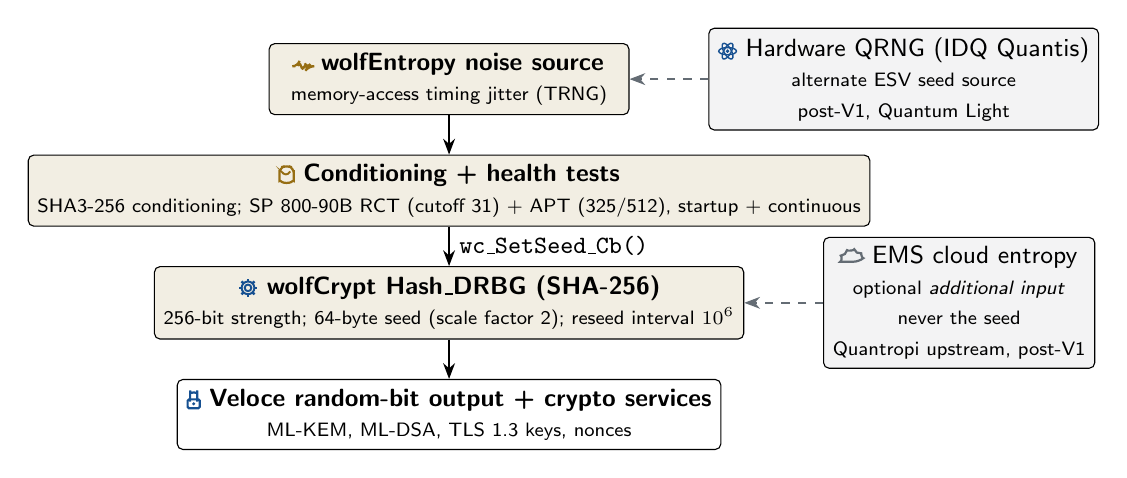
\begin{tikzpicture}[
  font=\small\sffamily,
  box/.style={draw, rounded corners=2pt, minimum height=2.4em, minimum width=13em, align=center, fill=white},
  arrow/.style={-{Stealth[length=2mm]}, thick},
  node distance=0.5cm]
  \node[box, fill=fipsgold!12] (src) {\icWave\ \textbf{wolfEntropy noise source}\\\scriptsize memory-access timing jitter (TRNG)};
  \node[box, fill=fipsgold!12, below=of src] (cond) {\icShield\ \textbf{Conditioning + health tests}\\\scriptsize SHA3-256 conditioning; SP 800-90B RCT (cutoff 31) + APT (325/512), startup + continuous};
  \node[box, fill=fipsgold!12, below=of cond] (drbg) {\icGear\ \textbf{wolfCrypt Hash\_DRBG (SHA-256)}\\\scriptsize 256-bit strength; 64-byte seed (scale factor 2); reseed interval $10^6$};
  \node[box, below=of drbg] (out) {\icLock\ \textbf{Veloce random-bit output + crypto services}\\\scriptsize ML-KEM, ML-DSA, TLS 1.3 keys, nonces};
  \node[box, right=1.0cm of drbg, minimum width=9em, fill=lrgray!8] (ems) {\icCloud\ EMS cloud entropy\\\scriptsize optional \emph{additional input}\\\scriptsize never the seed\\\scriptsize Quantropi upstream, post-V1};
  \node[box, right=1.0cm of src, minimum width=9em, fill=lrgray!8] (qrng) {\icAtom\ Hardware QRNG (IDQ Quantis)\\\scriptsize alternate ESV seed source\\\scriptsize post-V1, Quantum Light};
  \draw[arrow] (src) -- (cond);
  \draw[arrow] (cond) -- node[right]{\scriptsize \code{wc\_SetSeed\_Cb()}} (drbg);
  \draw[arrow] (drbg) -- (out);
  \draw[arrow, dashed, lrgray] (ems) -- (drbg);
  \draw[arrow, dashed, lrgray] (qrng) -- (src.east);
\end{tikzpicture}
\end{center}

\textbf{Wiring.} The module itself makes no entropy claim; the agent installs the entropy
source with \code{wc\_SetSeed\_Cb()} immediately after \code{wolfCrypt\_SetCb\_fips()} at
startup, backed by \code{wc\_Entropy\_Get()}. Each instantiate/reseed requests 64 bytes at
256-bit strength. The build uses \code{-{}-enable-wolfEntropy=nofallback} so the source can
\emph{never} silently fall back to \code{/dev/urandom} in FIPS mode.

\textbf{Fail-closed policy.} If entropy initialization, a health test (RCT/APT), or a
reseed fails, the agent transitions to a degraded state: all key generation, signing,
encapsulation, and TLS handshakes are refused; \code{health()} and the validation-status
API report the failure; an event-log entry and (if enabled) an EMS alert are emitted.
There is no API that returns raw entropy, and entropy is never sent to EMS.

\textbf{ESV evidence.} \code{wc\_Entropy\_GetRawEntropy()} provides raw noise samples for
SP~800-90B assessment. \dep{Confirm with wolfSSL the ESV certificate number and its
applicability to our exact Windows 11 x86-64 and Linux x86-64 operating environments;
entropy validations are OE-bound.}

\textbf{Entropy providers.} V1 ships exactly one credited entropy provider: the
wolfEntropy software source (ESV-verified). No hardware entropy is integrated in V1.
Two quantum-entropy integrations follow post-V1: the \textbf{Quantropi} quantum-entropy
service (QiSpace SEQUR), delivered over the network through the EMS cloud-entropy
channel as DRBG additional input (Section~\ref{sec:cloud-entropy}); and the IDQ Quantis
QRNG as a local alternate ESV seed source for Quantum Light deployments.
\code{list\_entropy\_providers()} enumerates providers, so new sources are added without
API change.

\subsection{FIPS module integration}
\begin{itemize}
  \item Module: wolfCrypt FIPS 140-3 v5.2.1, CMVP cert \#4718; library wolfSSL 5.9.2.
        Built with \code{-{}-enable-fips=v5} via autotools (CMake is not FIPS-capable in
        this tree). Loaded as a shared library / DLL, never statically linked; protected
        module files are never renamed, patched, or recompiled without wolfSSL approval.
  \item In-core integrity: HMAC-SHA256 check; build flow is
        \code{configure} $\rightarrow$ \code{make} $\rightarrow$ \code{./fips-hash.sh}
        $\rightarrow$ \code{make} $\rightarrow$ \code{testwolfcrypt} (Appendix~\ref{app:build}).
  \item Self-tests: power-on self-test at load plus conditional algorithm self-tests
        (CASTs) for AES-CBC/GCM, HMAC-SHA-1/2/3, DRBG, RSA sign, ECDSA, ECC-CDH, DH-Z,
        and the TLS 1.2/1.3/SSH KDFs. The SDK's \code{run\_fips\_self\_tests()} calls
        \code{wc\_RunAllCast\_fips()}, and status is read from
        \code{wolfCrypt\_GetStatus\_fips()}.
  \item Record for every build: DLL/so hash, source version, build settings, compiler,
        FIPS certificate, ESV certificate, operating environment (feeds the CBOM).
  \item Certificate \#4718 lists \textbf{Windows 11 Pro x86-64} (Intel Core i7-1255U)
        and Windows Server 2022 among its tested operational environments, alongside
        RHEL, Ubuntu, and Debian x86-64; wolfSSL support confirms this source package
        also builds the Windows module via the \code{IDE/WIN10} Visual Studio solution.
        The CMVP entry carries the caveat ``no assurance of the minimum strength of
        generated SSPs''; entropy assurance therefore comes solely from the ESV
        source. \dep{Confirm with wolfSSL: (a) the approved Windows \emph{DLL} build
        configuration (\code{IDE/WIN10} ships static-library settings, while the SDK
        requires dynamic loading); (b) the \code{user\_settings.h} variant matching
        module v5.2.1.}
\end{itemize}

\subsection{PQC provider outside the FIPS boundary}\label{sec:pqc-boundary}
The \#4718 boundary contains classical algorithms only, and this FIPS build strips the
SHAKE/XOF primitives that ML-KEM and ML-DSA require, so \textbf{PQC cannot link inside
the v5 FIPS build}. V1 therefore compiles the wolfSSL ML-KEM/ML-DSA sources (FIPS 203/204,
with fault-hardening flags) as a separate \emph{PQC provider} library beside the boundary,
drawing all randomness from the FIPS DRBG via the \code{*WithRandom} APIs.

\begin{itemize}
  \item Validation status reports each fact separately (no generic \code{FIPS=True}):
        module validated + cert number; entropy ESV validated + cert number; PQC algorithm
        and its validation status; \code{pqc\_inside\_fips\_boundary:\ false}; OE;
        self-test results. Values come from the installed module, never hardcoded.
  \item \dep{Track wolfSSL's FIPS v7 ``PQ-FS'' submission (boundary wrappers for ML-KEM,
        ML-DSA, LMS, XMSS, SLH-DSA + SHA-512 DRBG). Migrating to v7 flips
        \code{pqc\_inside\_fips\_boundary} to true with no API change; the provider
        interface is designed for that swap.}
  \item CAVP/ACVTS testing of the PQC provider (known-answer + interface tests) is planned
        so the CBOM can cite algorithm-level evidence even before v7.
        \open{Choose ACVTS scope and lab.}
\end{itemize}

\subsection{Hybrid TLS 1.3}
Sample client and server negotiate a wolfSSL-supported hybrid group. Candidates:
\code{X25519MLKEM768} (default), \code{SecP256r1MLKEM768}, \code{SecP384r1MLKEM1024}.
The public API accepts a \emph{policy profile}, never raw algorithm strings:

\begin{quote}
\code{session = veloce.tls.connect(host=..., port=443, policy="LIGHTRIDER\_PQC\_TRANSITION")}
\end{quote}

\dep{Do not hardcode the production group until wolfSSL confirms the group supported by
the licensed bundle, its validation status, the approved build configuration, and
interoperability expectations.}

\subsection{Performance plan}
Performance is verified by measurement. Using
\code{wolfcrypt/benchmark} plus Veloce-level harnesses, each release publishes:
DRBG throughput (MB/s, single and multi-threaded via per-thread RNG instances);
entropy source fill rate; ML-KEM-768 keygen/encap/decap ops/s; ML-DSA sign/verify ops/s;
hybrid TLS 1.3 handshakes/s; IPC round-trip latency. The baseline is captured at stage S1
on the reference environments; release gate = published performance report with no
regression $>$10\% against baseline. \open{Absolute targets to be set from the S1
baseline.}

% =====================================================================
\section{Pillar C: EMS Cloud Integration}\label{sec:ems}

EMS (\code{light-rider-platform}) is strictly optional. Veloce is fully functional with
EMS disabled; this default is enforced by a zero-network-traffic test.

\subsection{Modes and configuration}
\begin{quote}
\code{ems:\ \{ mode:\ disabled \}} \hfill or \hfill
\code{ems:\ \{ mode:\ enabled, endpoint:\ https://..., entropy\_mixin:\ off|on \}}
\end{quote}

\begin{small}
\begin{tabularx}{\textwidth}{@{}lL@{}}
\toprule
\textbf{EMS may receive} & Agent health; SDK and module versions; CBOM records; policy
  identifiers; self-test status; entropy-provider status; non-sensitive operational
  telemetry \\
\textbf{EMS must never receive} & Private keys; shared secrets; \emph{raw entropy}; DRBG
  seeds or state; unencrypted customer data; TLS session secrets \\
\bottomrule
\end{tabularx}
\end{small}

Transport: mTLS (hybrid TLS 1.3 once EMS supports it), device enrollment issuing a
per-device identity; the agent is the only component that opens the connection.
\open{EMS endpoint contract (REST vs gRPC), enrollment flow, and payload schemas are
designed at stage S3 jointly with the platform team.}

\subsection{User-controllable cloud entropy (V1 addition)}\label{sec:cloud-entropy}
EMS may deliver entropy \emph{to} devices; devices never send entropy to EMS.

\textbf{Design.}
\begin{enumerate}
  \item The agent (when \code{entropy\_mixin:\ on}) periodically fetches an authenticated,
        freshness-checked entropy packet from EMS over mTLS.
  \item The packet is injected into the wolfCrypt DRBG as SP~800-90A
        \emph{additional input} on reseed/generate: it is cryptographically mixed in but
        contributes \emph{zero} to the credited entropy claim. The local wolfEntropy ESV
        source remains the sole seed. The FIPS and ESV certificates are unaffected.
  \item User control: enable/disable per config or at runtime via the SDK
        (\code{set\_entropy\_mixin(...)}); state is visible in \code{health()},
        \code{list\_entropy\_providers()}, validation status, and the CBOM
        (\code{cloud\_entropy\_mixin:\ on/off}).
  \item Fail-safe: EMS unreachable, stale, or malformed packets $\Rightarrow$ mix-in is
        skipped and local operation continues untouched; a status flag records the last
        successful mix-in. Cloud entropy can never block or degrade local crypto.
\end{enumerate}
Post-V1, the same delivery channel carries quantum-sourced entropy: the Quantropi
quantum-entropy service (QiSpace SEQUR) as the EMS upstream source, and Quantum Light
QPU-derived entropy.

% =====================================================================
\section{APIs and Deliverables}\label{sec:api}

\subsection{Public Python API (17 functions, fixed by the guidance)}
\begin{small}
\begin{tabularx}{\textwidth}{@{}lL@{}}
\toprule
\textbf{Group} & \textbf{Functions} \\
\midrule
Lifecycle & \code{initialize()}, \code{health()}, \code{version()} \\
Discovery & \code{list\_policy\_profiles()}, \code{list\_crypto\_providers()},
  \code{list\_entropy\_providers()}, \code{validation\_status()} \\
ML-KEM & \code{mlkem\_generate\_keypair()}, \code{mlkem\_encapsulate()},
  \code{mlkem\_decapsulate()} \\
ML-DSA & \code{mldsa\_sign()}, \code{mldsa\_verify()} \\
TLS / FIPS & \code{configure\_hybrid\_tls()}, \code{run\_fips\_self\_tests()},
  \code{approved\_mode\_status()} \\
Reporting & \code{export\_cbom()}, \code{generate\_diagnostic\_bundle()} \\
\bottomrule
\end{tabularx}
\end{small}

Private keys never cross the IPC channel: key APIs return a public key plus an opaque
\code{private\_key\_handle}. V1 adds one extension pair for the approved scope change:
\code{set\_entropy\_mixin()} / mix-in status inside \code{list\_entropy\_providers()}.

\subsection{Deliverables checklist}
Python wheel (\code{veloce\_pqc-<ver>-py3-none-any.whl}); native agent; wolfCrypt shared
library/DLL; qSearch binary; Windows MSI (Authenticode-signed, service registration,
named-pipe ACLs, EMS-disabled default config, upgrade/repair/uninstall) and Linux
deb/rpm (systemd unit, socket permissions); CLI; API reference; architecture document;
security guide; FIPS integration guide; entropy-provider guide; SBOM and CBOM; sample TLS
client/server; test vectors; performance report; known-limitations statement; reseller
evaluation package; \textbf{Lightrider EULA} and \textbf{third-party notices file}
(wolfSSL attribution + collector licenses; see Section~\ref{sec:license}); branding
assets (logo artwork + ASCII banner, Section~\ref{sec:branding}).

\subsection{Startup branding}\label{sec:branding}

Client-visible entry points display Lightrider branding at startup. The banner's status
line is populated from \code{validation\_status()} at runtime, never hardcoded.

\begin{quote}
\begin{verbatim}
__   _____ _    ___   ___ ___
\ \ / / __| |  / _ \ / __| __|
 \ V /| _|| |_| (_) | (__| _|
  \_/ |___|____\___/ \___|___|
Lightrider Inc -- Veloce PQC SDK v<version>
FIPS 140-3 #4718 | ESV entropy: OK | approved mode: on
\end{verbatim}
\end{quote}

\begin{small}
\begin{tabularx}{\textwidth}{@{}lL@{}}
\toprule
\textbf{Surface} & \textbf{Behavior} \\
\midrule
Veloce CLI & Prints the ASCII banner + status line on interactive startup. Suppressed
  when stdout is not a TTY, with \code{-{}-quiet} or \code{-{}-json}, or when
  \code{VELOCE\_NO\_BANNER=1}; machine-readable output is never polluted. \\
Veloce Agent & Writes the banner and status line to its startup log entry: Windows
  Event Log source on Windows, journald/syslog on Linux. \\
Python SDK & No output on \code{import} (library convention); banner available
  explicitly via \code{veloce.banner()}. \\
Installers & MSI UI dialogs carry Lightrider logo artwork; deb/rpm post-install prints a
  one-line branded confirmation with version and FIPS certificate. \\
Reports & CBOM exports, diagnostic bundles, and the qSearch executive summary carry a
  product-identity header (name, version, certificates). \\
\bottomrule
\end{tabularx}
\end{small}

Branding assets live in \code{assets/branding/} (logo SVG/ICO for installers and
documentation; \code{banner.txt} as the single source for the ASCII art).

% =====================================================================
\section{Security and Compliance}\label{sec:security}

\begin{small}
\begin{tabularx}{\textwidth}{@{}lL@{}}
\toprule
\textbf{Control area} & \textbf{V1 implementation} \\
\midrule
Key custody & All private keys and sensitive state live in the agent; opaque handles
  outside; zeroization on release (tested). \\
IPC hardening & Windows: named pipe \code{\textbackslash\textbackslash.\textbackslash
  pipe\textbackslash LightRider.PQC.v1} with an explicit ACL (service identity, authorized
  local user, local admins; deny anonymous/remote/unauthenticated; never the default
  descriptor). Linux: UNIX domain socket, mode 0660, \code{SO\_PEERCRED} checks.
  Versioned length-prefixed protocol; no raw entropy, DRBG state, keys, or plaintext
  diagnostics on the channel. \\
Library loading & Windows: absolute path under \code{Program Files},
  \code{SetDefaultDllDirectories} + \code{LoadLibraryExW} restricted search; never in
  \code{System32} or global \code{PATH}. Linux: absolute \code{dlopen} path, no
  \code{LD\_LIBRARY\_PATH} trust; DLL/so hash verified against the recorded build hash. \\
Service identity & Windows service \code{VelocePqcAgent} under
  \code{NT AUTHORITY\textbackslash LocalService}; Linux systemd unit with a dedicated
  low-privilege user, \code{ProtectSystem=strict}. \dep{Confirm service-account choice
  against wolfSSL operational-environment requirements.} \\
Certificates reported & FIPS 140-3 cert \#4718 (module v5.2.1) + ESV entropy certificate,
  each bound to its exact OE; surfaced in validation status and CBOM. \\
Data hygiene & Diagnostic bundles are redaction-tested; CBOM output contains metadata
  only: never keys, seeds, passwords, tokens, or customer plaintext (mirrors the CBOM
  workbook rule). \\
Supply chain & Licensed wolfSSL source confined to a restricted private repo
  (\code{vendor/}); reproducible FIPS builds; signed installers; SBOM per release;
  qSearch collector licenses vetted (Apache-2.0/MIT/BSD). \\
\bottomrule
\end{tabularx}
\end{small}

\subsection{Licensing and distribution model}\label{sec:license}

Lightrider holds a wolfSSL commercial license (Agreement v.01-24 in the bundle);
\textbf{Veloce ships under Lightrider's own commercial license (EULA)}, wrapping wolfCrypt
as an embedded component. The agreement's terms impose the following requirements:

\begin{small}
\begin{tabularx}{\textwidth}{@{}>{\raggedright\arraybackslash}p{0.40\textwidth}L@{}}
\toprule
\textbf{Agreement fact} & \textbf{What Veloce must do} \\
\midrule
\S3: distribute the ``Combined Program'' in \emph{object code} only &
  Ship wolfCrypt exclusively as the compiled DLL/\code{.so} inside Veloce installers:
  never source, never as a standalone library. Already matched by the dynamic-library
  design and the restricted \code{vendor/} repo. \\
\S3: license is contingent on the Combined Program \emph{not} being a cryptography
  library that competes with the Products &
  \dep{Confirm with wolfSSL that Veloce (a PQC SDK exposing crypto \emph{services}
  through the local agent, not an embeddable crypto library) is the named Program on the
  Order Form.} Supporting position: Veloce exposes cryptographic services through the
  local agent (opaque handles), not a linkable crypto library. \\
\S3: per-Developer licensing (anyone who links, compiles, or edits code using the
  Products) &
  Count agent/core developers against the Order Form seat count; qSearch and Python SDK
  developers never touch wolfCrypt and do not count. Track seats in the repo access list. \\
\S4: retain wolfSSL copyright notices; attribution in documentation permitted;
  no sublicense/transfer &
  Keep wolfSSL notices in the shipped binaries and a \textbf{third-party notices file};
  docs state Veloce is ``built with wolfCrypt (FIPS 140-3 cert \#4718)''. The Lightrider
  EULA licenses \emph{Veloce}, and must not purport to sublicense wolfSSL itself. \\
\S5: confidentiality (3 years / trade-secret duration) &
  FIPS source bundle and build configs stay in the restricted private repo; excluded from
  any public repository and from customer deliveries (including the
  Customer Operational-Environment Package). \\
\S7: end-user rights survive termination &
  End-user license continuity is reflected in the Lightrider EULA. \\
\S10: support covers updates to the licensed version, not upgrades &
  \dep{The FIPS v7 ``PQ-FS'' migration is an \emph{upgrade}; budget a new
  wolfSSL Order Form for it.} \\
\S11: FAR 12.211/12.212, DFARS 252.227-7015 government rights &
  Mirror the restricted-rights language in the Lightrider EULA; required for the
  M-23-02 federal customer base. \\
\bottomrule
\end{tabularx}
\end{small}

Layered result: \textbf{Lightrider EULA} (Veloce SDK, all Lightrider-owned code)
$\rightarrow$ \textbf{wolfSSL commercial license} (embedded wolfCrypt object code,
invisible to the customer beyond notices) $\rightarrow$ \textbf{permissive licenses}
(Apache-2.0/MIT/BSD qSearch collectors, listed in the notices file). qSearch and the
Python SDK contain no wolfSSL code, so Lightrider may license them freely under its own
terms.

% =====================================================================
\section{Test Gates and Acceptance}\label{sec:gates}

Release is gate-based: V1 does not ship until every gate passes on both platforms.

\begin{small}
\begin{tabularx}{\textwidth}{@{}lL@{}}
\toprule
\textbf{Gate group} & \textbf{Must pass} \\
\midrule
FIPS \& entropy & wolfCrypt test suite; startup + conditional self-tests; wolfEntropy
  init and health tests; induced entropy-failure and reseed-failure tests (fail-closed
  verified); DRBG continuous-test behavior. \\
PQC & ML-KEM keygen/encap/decap and ML-DSA sign/verify known-answer tests; fault-harden
  builds; negative tests (corrupted ciphertext/signature). \\
TLS & Hybrid TLS 1.3 client/server interop; negotiated-group reporting; certificate
  validation; downgrade rejection; fragmented handshakes; unsupported-server behavior;
  EMS on/off operation. \\
IPC \& platform & Named-pipe/socket authorization; unauthorized-local-user rejection;
  remote-access rejection; DLL substitution and search-path attacks; key zeroization;
  diagnostic redaction. \\
EMS & Zero network traffic when disabled; telemetry allow-list enforcement when enabled;
  entropy mix-in on/off behavior incl.\ EMS-unavailable fail-safe. \\
qSearch & Controlled sample environments containing known RSA, ECDH, ECDSA, DH, ML-KEM,
  ML-DSA implementations: expected detections found; false positives and blind spots
  explicitly reported; CBOM accuracy vs.\ ground truth; CycloneDX schema validation;
  offline-mode run. \\
Packaging \& perf & MSI install/upgrade/repair/uninstall; deb/rpm equivalents;
  config preserved across upgrades; performance and memory benchmarks published. \\
\bottomrule
\end{tabularx}
\end{small}

\textbf{V1 completion criteria} (condensed): Python SDK talks only through the agent;
wolfCrypt loaded dynamically; ESV source seeds the DRBG; hybrid TLS works client/server;
full local operation with EMS disabled; EMS enable exposes no secrets; validation status
accurate per-item; CBOM export automatic; installers produce securely configured
services; all gates green.

% =====================================================================
\section{Execution Guide: What To Do, In Order}\label{sec:schedule}

Work proceeds as a dependency-ordered sequence of stages, each closed by an objective
gate. The two pillars run in parallel after S0. Vendor items (\dep{}) are on the critical
path and are opened at S0.

\begin{small}
\begin{tabularx}{\textwidth}{@{}llL@{}}
\toprule
\textbf{Stage} & \textbf{Target} & \textbf{What to do / exit gate} \\
\midrule
S0 & Foundations & Repo + CI skeleton; Linux FIPS build brought up
  (\code{-{}-enable-fips=v5 -{}-enable-wolfEntropy=nofallback}, fips-hash flow,
  \code{testwolfcrypt} green); IPC protocol v1 drafted; wolfSSL engagement opened
  (Windows DLL build configuration, ESV cert applicability, hybrid group, v7 timeline).
  \emph{Gate G0: FIPS module passes self-tests on the Linux reference machine.} \\
S1 & Entropy + core & Agent skeleton (Linux daemon + Windows
  service); wolfEntropy wired via \code{wc\_SetSeed\_Cb}; fail-closed state machine;
  PQC provider built beside boundary + KATs; validation-status API; performance baseline.
  \emph{Gate G1: entropy pipeline + ML-KEM/ML-DSA pass all KATs and failure-injection
  tests on both OSes.} \\
S2 & qSearch & Rust engine + finding schema; source/dependency/
  certificate collectors; Zeek/PCAP pipeline (Linux native, Windows capture);
  classification + CBOM (JSON/CSV/CycloneDX); sample-environment accuracy runs.
  \emph{Gate G2: qSearch detects all planted crypto in the controlled environments and
  reports false positives/blind spots.} (Parallel to S1.) \\
S3 & TLS + EMS & Hybrid TLS 1.3 samples + interop; Python SDK
  surface complete; CLI; EMS telemetry client + enrollment; cloud-entropy mix-in;
  zero-traffic verification. \emph{Gate G3: TLS + EMS gate groups green.} \\
S4 & Harden \& ship & Full security test battery (IPC, DLL, zeroization,
  redaction); packaging (MSI, deb/rpm, wheel); docs set; performance report;
  known-limitations statement; reseller evaluation package.
  \emph{Gate G4 = V1 release candidate.} \\
\bottomrule
\end{tabularx}
\end{small}

\subsection{Component-to-repository traceability}

Each repository directory implements a specification section and is accepted by an
exit gate.

\begin{small}
\begin{tabularx}{\textwidth}{@{}lLl@{}}
\toprule
\textbf{Repository path} & \textbf{Specification} & \textbf{Gate} \\
\midrule
\code{vendor/wolfssl/} & Appendix~\ref{app:build} build recipes;
  \S\ref{sec:license} license constraints & G0 \\
\code{ipc/} & \S\ref{sec:arch} IPC protocol; \S\ref{sec:security} channel ACLs & G1 \\
\code{agent/} & \S\ref{sec:core} entropy pipeline, FIPS integration, PQC provider;
  \S\ref{sec:security} key custody, loading, service identity & G1 \\
\code{qsearch/} & \S\ref{sec:qsearch} collectors, finding format, outputs & G2 \\
\code{cbom/} & \S\ref{sec:qsearch} output formats; Appendix~\ref{app:cbom} field
  mapping & G2 \\
\code{python/} & \S\ref{sec:api} API surface; \S\ref{sec:ems} EMS controls & G3 \\
\code{cli/} & \S\ref{sec:api} operator commands; \S\ref{sec:branding} banner & G3 \\
\code{examples/} & \S\ref{sec:core} hybrid TLS 1.3 client/server & G3 \\
\code{tests/} & \S\ref{sec:gates} gate definitions & G0--G4 \\
\code{installer/} & \S\ref{sec:api} packaging; \S\ref{sec:security} secure defaults & G4 \\
\code{assets/branding/} & \S\ref{sec:branding} logo + banner assets & G4 \\
\code{docs/} & \S\ref{sec:api} documentation deliverables & G4 \\
\bottomrule
\end{tabularx}
\end{small}

Post-V1 roadmap: wolfSSL FIPS v7 migration (PQC inside boundary); IDQ Quantis QRNG as
alternate local ESV seed source (Quantum Light); Quantropi QiSpace SEQUR entropy as the
EMS upstream, delivered over the mix-in channel; QPU-derived cloud entropy;
macOS; multi-source entropy pooling; qSearch remediation orchestration.

% =====================================================================
\section{Risks and Open Items}\label{sec:risks}

\begin{small}
\begin{tabularx}{\textwidth}{@{}Lll L@{}}
\toprule
\textbf{Risk / item} & \textbf{Prob.} & \textbf{Impact} & \textbf{Mitigation} \\
\midrule
Windows FIPS \emph{DLL} configuration + ESV OE applicability unconfirmed by wolfSSL
  (cert \#4718 itself already lists Windows 11 Pro x86-64 as a tested OE) & M & M &
  Engage at S0; Linux track proceeds independently; Windows gates depend only on S1+. \\
PQC outside FIPS boundary until v7 & certain & M & Honest per-item status reporting
  (already the documented design); ACVTS algorithm evidence; v7 migration path built into
  the provider interface. \\
PQC implementation defects (cf.\ CVE-2026-6330, ML-KEM ARM64 ciphertext-comparison flaw)
  & L--M & H & Stay current with wolfSSL releases; KAT + negative tests in CI; x86-64-only
  scope in V1 limits exposure. \\
Hybrid TLS production group unconfirmed & M & M & Policy-profile indirection means the
  group is config, not API; default \code{X25519MLKEM768} pending confirmation. \\
wolfSSL \S3 compete clause: Veloce could be read as a ``cryptography library'' & M & H &
  Paper Veloce as the named Program on the Order Form at S0; agent-service architecture
  (no linkable crypto API) is the supporting position; legal review of the Lightrider
  EULA wrap. \\
Collector licensing (GPL) blocks bundling & M & M & Legal review at S0; adapters keep
  collectors replaceable; bring-your-own-collector fallback. \\
wolfEntropy throughput insufficient for high-rate workloads & M & M & Per-thread DRBG
  instances (reseeds amortized); measure at the S1 baseline; QRNG roadmap as high-rate
  alternative. \\
Federal CBOM minimum elements published mid-project & M & L & Versioned CBOM schema
  module; workbook already flags mandatory update on issuance. \\
Zeek-on-Windows immaturity & certain & L & Documented capture-and-forward design
  (TShark/Npcap $\rightarrow$ Linux/WSL sensor); native Windows analysis revisited post-V1. \\
\bottomrule
\end{tabularx}
\end{small}

% =====================================================================
\appendix

\section{Build Recipes}\label{app:build}

\subsection*{Linux FIPS module (bundle on hand)}
\begin{quote}
\code{cd vendor/wolfssl}\\
\code{./configure -{}-enable-fips=v5 -{}-enable-wolfEntropy=nofallback}\\
\code{make}\\
\code{./fips-hash.sh}\quad\emph{\small(updates the in-core HMAC-SHA256 verify hash)}\\
\code{make}\\
\code{./wolfcrypt/test/testwolfcrypt}\quad\emph{\small(must report all tests passed)}
\end{quote}
Notes: autotools is the only FIPS-capable build path in this tree; \code{-{}-enable-fips}
also turns on reproducible builds. Record DLL/so SHA-256, source version, compiler, and
flags into the CBOM store at build time.

\subsection*{PQC provider (beside boundary)}
Separate non-FIPS build of the same wolfSSL tree (or standalone compilation of
\code{wc\_mlkem.*} and \code{wc\_mldsa.*} with SHAKE enabled), configured with
\code{-{}-enable-mlkem -{}-enable-mldsa} plus the fault-hardening flags
\code{WC\_MLKEM\_FAULT\_HARDEN} and \code{WC\_MLDSA\_FAULT\_HARDEN}; randomness supplied
exclusively from the FIPS DRBG via the \code{*WithRandom} APIs; distinct library name and
symbol namespace so the two builds can never be confused at load time.

\subsection*{Windows}
Use the wolfSSL-provided \code{IDE/WIN10} FIPS solution (\code{wolfssl-fips.sln}),
Platform \code{x64}, per-wolfSSL-approved configuration only; wolfSSL support confirms
this source package also builds the Windows module, and cert \#4718 lists Windows 11 Pro
x86-64 as a tested OE. \dep{Approved DLL configuration and \code{user\_settings.h}
variant to be confirmed.} Then follow the same hash-verify-record flow.

\section{CBOM Field Mapping (SDK $\rightarrow$ workbook)}\label{app:cbom}

The Veloce agent's self-report and qSearch findings both flow into the Light Rider CBOM
workbook schema:

\begin{small}
\begin{tabularx}{\textwidth}{@{}lL@{}}
\toprule
\textbf{Veloce report field} & \textbf{CBOM Inventory column} \\
\midrule
Crypto library / module + version & Crypto Library/Provider; Library Version;
  Cryptographic Module \\
FIPS certificate (\#4718) & FIPS 140-3 Certificate \\
Entropy provider + ESV certificate & Entropy Source; ESV Status/Certificate \\
Algorithm + parameter set (e.g.\ ML-KEM-768) & Algorithm; Key/Parameter Size;
  Target PQC Algorithm \\
TLS version + hybrid group & Protocol/Version; Cipher Suite \\
Approved-mode + self-test status & Notes / runtime validation record \\
OS edition, build, CPU arch & Operating System (Supplier sheet); Environment \\
qSearch finding provenance + confidence & Discovery Findings: Discovery Method, Finding
  Confidence, Validation Status, False Positive?, Blind Spot/Limitation \\
Scan runs & Scanning Log sheet (tool/method, findings counts, false positives) \\
\bottomrule
\end{tabularx}
\end{small}

Additional SDK-only CBOM fields (JSON/CSV export): agent version, wolfCrypt DLL/so name +
SHA-256, EMS enabled/disabled, cloud-entropy mix-in state, installation and last-verified
timestamps.

\section{References}\label{app:refs}

\begin{small}
\begin{enumerate}
  \item OMB Memorandum M-23-02, \emph{Migrating to Post-Quantum Cryptography} (Nov 2022).
  \item CISA, \emph{Strategy for Migrating to Automated Post-Quantum Cryptography
        Discovery and Inventory Tools} (Sep 2024).
  \item CISA, \emph{2026 Minimum Elements for a Software Bill of Materials} (Jul 2026).
  \item NIST FIPS 203 (ML-KEM), FIPS 204 (ML-DSA); FIPS 140-3; SP 800-90A/B.
  \item NIST CMVP validated-modules search (wolfSSL):\\
        \url{https://csrc.nist.gov/projects/cryptographic-module-validation-program}.
  \item CryptoScan: \url{https://github.com/csnp/cryptoscan}; Zeek packet analysis:
        \url{https://docs.zeek.org}.
  \item wolfSSL 5.9.2 release (Jun 23, 2026), commercial FIPS bundle
        \code{linuxv5.2.1}; wolfSSL FIPS-FAQ v2.3.
  \item Minimus, \emph{From SBOM to CBOM} and \emph{How to Use CBOMs in Containerized
        Environments} (industry perspective).
  \item Light Rider CBOM Starter Template (\code{Light\_Rider\_CBOM\_Template\_Updated.xlsx}).
\end{enumerate}
\end{small}

\end{document}
